%!TEX root = ../../adrien_gomar_phd.tex

Originally developed by \citet{He1998} and \citet{Ning1998},
the NLH method
relies on a decomposition of the conservative variables into a
time-averaged part plus an unsteady perturbation:
\begin{equation}
	u = \overline{u} + u^\prime,
	\label{eq:sm_nlh_decomposition}
\end{equation}
where $\overline{.}$ denotes the time-averaging operator and
$.^\prime$ its unsteady perturbation counterpart.
By injecting Eq.~\ref{eq:sm_nlh_decomposition} into
Eq.~\ref{eq:sm_nonlinear_convection_conservative}, one gets:
\begin{equation}
	\frac{\partial u^\prime}{\partial t} + 
	\frac{1}{2}\frac{\partial}{\partial x} \left[
	\overline{u}^2 + 2 \overline{u} u^\prime + u^\prime u^\prime \right] = 
	0.
	\label{eq:sm_nlh_step_1}
\end{equation}
The time-averaged equation can be obtained by time-averaging
equation~\ref{eq:sm_nlh_step_1}:
\begin{equation}
	(\overline{\ref{eq:sm_nlh_step_1}})
	\Leftrightarrow
	\frac{\partial}{\partial x}
	\left[\overline{u}^2 + 
	\overline{u^\prime u^\prime}\right] =
	0,
	\label{eq:sm_nlh_step_2}
\end{equation}
The term $\overline{u^\prime u^\prime}$
appears due to the non-linearities of the considered equation. It
is called the nonlinear stress terms 
(or the deterministic stress terms) as a reference to 
the Reynolds stress terms. 
The equation for the unsteady perturbations is then obtained by keeping
the first order terms of the unsteady equation~\ref{eq:sm_nlh_step_1}.
This means that the term $u^\prime u^\prime$ is neglected and leads
to:
\begin{equation}
	\frac{\partial u^\prime}{\partial t} + 
	\frac{\partial}{\partial x} \left[\overline{u} u^\prime \right] = 
	0.
\end{equation}

\paragraph{Mono-frequential formulation}
For now on, no assumption has been made neither on the velocity $u$,
nor on its time-averaged part and unsteady perturbation part.
Now, assuming that the velocity perturbation 
is periodic in time with period
$T=2 \pi / \omega$,
the unsteady perturbations can be decomposed into 
a Fourier series:
\begin{equation}
	u^\prime = \sum_{k=-\infty \atop k \neq 0}^{\infty} 
	\widehat{u}_k e^{i \omega k t}.
	\label{eq:sm_nlh_decomposition_pert}
\end{equation}
Hence, since the complex exponentials family forms 
an orthogonal basis, we have for all harmonics 
$-\infty \leq k \leq \infty, \; k \neq 0$:
\begin{equation}
	i \omega k \widehat{u}_k + 
	\frac{\partial}{\partial x} \left[ \overline{u} \widehat{u}_k\right] =
	0.
\end{equation}
One can notice that the time-averaged part has been removed from
the Fourier series through $k \neq 0$ as it is computed 
separately in Eq.~\ref{eq:sm_nlh_step_2}.
Each harmonic equation represents now a steady equation as no temporal
derivative is present anymore.

The term $\overline{u^\prime u^\prime}$ remains in the time-averaged
equation and needs to be computed. It can be 
directly worked out when the harmonics are known:
\begin{equation}
	\begin{split}
		u^\prime u^\prime &= 
		\left[
			\sum_{k=-\infty \atop k \neq 0}^{\infty} \widehat{u}_k e^{i \omega k t} 
		\right]
		\left[
			\sum_{k=-\infty \atop k \neq 0}^{\infty} \widehat{u}_k e^{i \omega k t} 
		\right] \\
		&= \sum_{k=-\infty \atop k \neq 0}^{\infty} (\widehat{u}_k)^2
		   e^{i 2 \omega k t} +
		   2 \sum_{j,k=-\infty \atop j \neq k \neq 0}^{\infty} 
		   \widehat{u}_k \widehat{u}_j e^{i \omega (j + k) t} \\
	\end{split}
\end{equation}
Thus,
\begin{equation}
	\begin{split}
		\overline{u^\prime u^\prime} &= 
		\frac{1}{T} \int_{t=0}^{T} \left[ 
			\sum_{k=-\infty \atop k \neq 0}^{\infty} (\widehat{u}_k)^2
		   	e^{i 2 \omega k t} +
		   	2 \sum_{j,k=-\infty \atop j \neq k \neq 0}^{\infty} 
		   	\widehat{u}_k \widehat{u}_j e^{i \omega (j + k) t} 
		\right] dt\\
		&= \frac{2}{T} \int_{t=0}^{T} \sum_{j,k=-\infty \atop j \neq k \neq 0}^{\infty} 
		   	\widehat{u}_k \widehat{u}_j 
		   	e^{i \omega (j + k) t} dt \\
		&= \frac{2}{T} \int_{t=0}^{T} 
			\sum_{k=-\infty \atop k \neq 0}^{\infty} 
			\widehat{u}_k \widehat{u}_{-k}  dt.
	\end{split}
\end{equation}
As $\widehat{u}_k$ and $\widehat{u}_{-k}$ are complex conjugates,
finally $\overline{u^\prime u^\prime}$ is equal to:
\begin{equation}
	\overline{u^\prime u^\prime} = 
	2 \sum_{k=-\infty \atop k \neq 0}^{\infty} |\widehat{u}_k|^2.
	\label{eq:sm_nlh_deterministic_stress_terms}
\end{equation}
This last equation depends only on the computed harmonics, meaning
that no term is modeled. Moreover, this term couples the
time-average solution with the unsteady perturbations. This is this
terms that is neglected in the linearized method seen in 
Sec.~\ref{sub:sm_lur}. This term takes into account for the 
non-linearity of the considered equation.

Finally, as computing an infinite number of harmonics is 
numerically not feasible,
the number of harmonics is truncated at order $N$. 
This is a fare assumption as most
of the physical flows have a finite unsteady spectrum. This
is for sure a reduce order approach. However, the goal of spectral
methods is to have a compact representation of the unsteady time
signals. As for a mesh grid convergence, the number of harmonics $N$
is increased until the unsteady representation of the signal is
converged for the variable of interest. The discussion on the
convergence of spectral methods will be detailed later on in this 
thesis \todo{ref chapitre}.

To summarize, the NLH
method applied to Eq.~\ref{eq:sm_nonlinear_convection_conservative},
gives $2N + 1$ equations. A pseudo-time ($\tau$) derivative is
added to march the equations in pseudo-time to the steady-state 
solution of all the harmonics:
\begin{equation}
	\fbox{$
	\begin{cases}
		\displaystyle \frac{\partial \overline{u}}{\partial \tau} + 
		\frac{\partial}{\partial x}
			\left[\overline{u}^2 + 
			\overline{u^\prime u^\prime}\right] &=
			0, \\
		\displaystyle \frac{\partial \widehat{u}_k}{\partial \tau} + 
		i \omega k \widehat{u}_k + 
			\frac{\partial}{\partial x} 
			\left[ \overline{u} \widehat{u}_k\right] &= 
			0, \: k \in [-N, N], \: k \neq 0,
	\end{cases}
	$}
	\label{eq:sm_nlh_subset_eq}
\end{equation}
coupled by the deterministic stress term $\overline{u^\prime u^\prime}$
defined in Eq.~\ref{eq:sm_nlh_deterministic_stress_terms}.
The term $u^\prime u^\prime$ is neglected in this formulation.

\paragraph{Multi-frequential formulation}

\citet{He2002} extended the method is extended to a multi-frequential
formulation. Instead of writing the perturbations
using a Fourier series as defined in Eq.~\ref{eq:sm_nlh_decomposition_pert},
these are written using a sum of harmonics each of which
having a frequency $\omega_k$:
\begin{equation}
	u^\prime = \sum_{k=-N \atop k \neq 0}^{N} 
	\widehat{u}_k e^{i \omega_k t}.
	\label{eq:sm_nlh_decomposition_pert_multi}
\end{equation}
Note that the term $k \omega$ in Eq.~\ref{eq:sm_nlh_decomposition_pert}
is now $\omega_k$ meaning that frequencies can be chosen
arbitrarily.
The derivation of the equations is kept the same and the following
$2N+1$ subset of equations is finally obtained:
\begin{equation}
	\fbox{$
	\begin{cases}
		\displaystyle
		\frac{\partial \overline{u}}{\partial \tau} +
		\frac{\partial}{\partial x}
			\left[\overline{u}^2 + 
			\overline{u^\prime u^\prime}\right] &=
			0, \\
		\displaystyle
		\frac{\partial \widehat{u}_k}{\partial \tau} + 
		i \omega_k \widehat{u}_k + 
			\frac{\partial}{\partial x} 
			\left[ \overline{u} \widehat{u}_k\right] &= 
			0, \: k \in [-N, N], \: k \neq 0.
	\end{cases}
	$}
	\label{eq:sm_nlh_subset_eq_multi}
\end{equation}
However, as the complex exponentials do not form
an orthogonal basis, writing Eq.~\ref{eq:sm_nlh_subset_eq_multi}
for each harmonic $k \in [-N, N], \: k \neq 0$ is mathematically
not true. \citet{He2002} argued that the terms
are collected for each harmonic. 
The same development is made by \citet{Vilmin2006}.

The coupling deterministic stress term is evaluated using the
same equation as for the mono-frequential formulation.
However, in the multi-frequential formulation, 
the equation Eq.~\ref{eq:sm_nlh_deterministic_stress_terms}
is generally not true.
In fact, in the mono-frequential formulation, the term
\begin{equation}
	\frac{1}{T} \int_{t=0}^{T} (\widehat{u}_k)^2
		e^{i 2 \omega k t} dt
	\label{eq:sm_nlh_int_deterministic}
\end{equation}
vanishes for each $k$ as the integral of the
exponential $e^{i 2 \omega k t}$ with respect to $t$
is given by $e^{i 2 \omega k t} / 2 i \omega k$ that is
periodic with period $T$ meaning that the integral in 
Eq.~\ref{eq:sm_nlh_int_deterministic} is equal to zero. 
However, in the multi-frequential
formulation, for some choice of frequencies, the period of all
of these may be difficult or even impossible to define. It
seems that mathematical justifications should be given
to be able to evaluate the deterministic stress term 
using Eq.~\ref{eq:sm_nlh_deterministic_stress_terms}.

\paragraph{Clocking effects}
\citet{He2002} extended the nonlinear harmonic method to
the computation of all clocking positions in one computation. Before
go into details of how this is done, let us explain what is
the clocking effect.
\begin{figure}[htbp]
  \centering 
  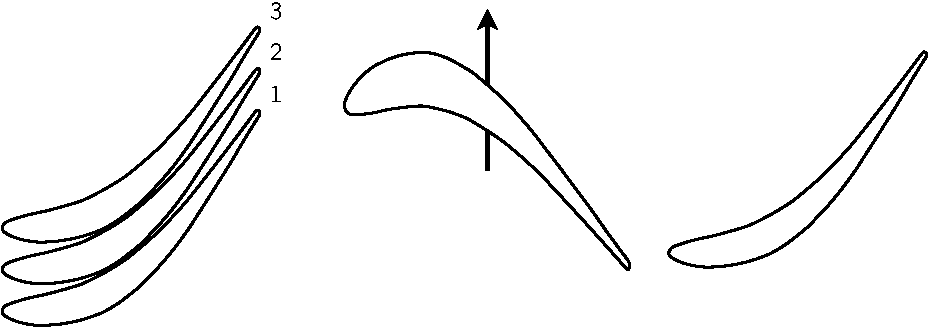
\includegraphics[width=.5\textwidth]{clocking_effect.pdf}
  \caption{Different clocking positions for a stator/rotor/stator
  configuration.}
  \label{fig:sm_nlh_clocking_effect}
\end{figure}
Fig.~\ref{fig:sm_nlh_clocking_effect} shows six
different clocking positions of the first stator
in a stator/rotor/stator configuration.
As both stator are fixed, their relative position is of 
prior interest. In fact, the wake that is generated behind the first stator
is cut by the rotor blades and transmitted to 
the stator row. The stator being fixed, the wake generated
behind the first stator is seen as a stationary wave in the second stator.
Hence, the importance of their relative position. For instance,
\citet{Huber1996} showed that
on their 1.5 turbine stage, the variation of efficiency due to clocking
effect was equal to $0.8\%$ of efficiency.

The brute force to compute the clocking effect on a
configuration is to consider all relative positions. This means
that the geometry of the stator should be rotated for each new 
clocking position. The innovative thinking proposed in 
\citet{He2002} is to consider the clocking effect as a steady wave.
In fact, as both stator are fixed, a steady perturbation
generated behind the first stator is still steady in the second stator.
In terms of frequencies, a steady perturbation is a perturbations 
whose frequency is zero. In \citet{He2002} and \citet{Vilmin2009}, 
a perturbation with zero frequency
is computed. The clocking effect can then be evaluated by
post-processing the Fourier coefficient of the zero frequency mode.
Recently, the computation of clocking effects on
arbitrary configurations has been made possible
by \citet{Vilmin2013a}.

\paragraph{Extension to the Navier-Stokes equations}
As shown above, as the development of the non-linear harmonic
method is made in the frequency domain, applying the method to
complex equations can be difficult. For the Navier-Stokes equations,
this step is particularly hard. Nevertheless, several authors have
done this and the reader is referred to the following papers
for more information~\cite{He1998, Chen2001, He2002, Vilmin2006}.

\paragraph{Time line}
\begin{figure}[htbp]
  \centering
  \includegraphics*[scale=0.5]{timeline_nlh.pdf}
  \caption{Time line for the non-linear harmonic method}
  \label{fig:timeline_nlh}
\end{figure}
Figure~\ref{fig:timeline_nlh} shows the time line of the
development of the non-linear harmonic method. 
Note that black filled
rectangles highlight multi-frequential formulation.
\citet{He1998}
and \citet{Ning1998} first introduced the method.
\citet{He1998} developed the method for the 
two-dimensional Reynolds-Averaged Navier-Stokes equations. 
While only one harmonic is
kept in the applications, the method is presented for multiple
harmonics. It is validated on an unsteady boundary layer
on a flat plate, a transonic diffuser with oscillating back pressure
and on an oscillating transonic compressor cascade.
\citet{Ning1998} developed the method on the two-dimensional
Euler equations with moving grids 
and applied it on a transonic unsteady
channel flow and on two cascade test cases
showing a good agreement with a classical non-linear
time-marching scheme. Emphasis is put on the capability
of the non-linear harmonic method to correctly capture
the unsteadiness in presence of strong non-linearities
compared to linearized methods (presented in 
Sec.~\ref{sub:sm_lur}).
\citet{Chen2001} extended the method to the three-dimensional
Navier-Stokes equations. Stage configurations are treated and
at the interface of the stage, the perturbations are exchanged using
azimuthal Fourier transform,
the time-average field and the deterministic stresses
being flux-averaged like in a mixing-plane approach.
\citet{He2002} extended the method
to take into account for the clocking effects. The frequencies
can be chosen arbitrarily allowing its application on multi-stage
turbomachines. The clocking effect is considered as a zero-frequency
temporal wave which is actually a spatial wave. The clocking
effect is then just analyzed through a post-processing procedure.
The method is applied on a $2.5$-stage transonic
compressor. The results are analyzed in terms of clocking effects
but not compared to neither classical non-linear time marching 
computations nor analytical simulations.
\citet{Vilmin2006} implemented the method into
the commercial code Fine/Turbo. They extended the rotor-stator
interface to a non-matching join sliding mesh interface which
leads to the continuity of the unsteady flow field at the interface.
The method is validated on analytical and $2$D test cases. Finally
a $4$-stage industrial transonic compressor is simulated to prove the 
maturity of the method.
\citet{Vilmin2007} extended the method to thermally perfect gas and
applied it to a $3$D real gas flow in a radial turbine and compared their
results to a classical time-marching simulation.
\citet{Vilmin2009} implemented and validated the clocking computation method
proposed by \citet{He2002}. They validated their approach on a model problem
and applied it
on a $2$D $6.5$-stage compressor and $1.5$-stage axial turbine.
\citet{Vilmin2013a} extended the row interface to take into
account in the third rotor for perturbations 
coming from the first rotor in an
arbitrary rotor/rotor/rotor configurations.

\paragraph{Cost of the method}
Compared to the LUR method, the number of equations to solve is 
not constant here. In fact, if $N$ denotes the number of harmonics
computed in total (sum of each harmonic of each perturbation)
then, if $\mathdollar_{\text{RANS}}$ 
denotes the CPU and memory cost of
one steady computation, one time-average equation and
$2N$ harmonic equations are solved, hence:
\begin{equation}
	\mathdollar_{\text{NLH}} = (2N+1) \cdot \mathdollar_{\text{RANS}}
\end{equation}
However, \citet{Vilmin2006} do not apply the NLH formulation
on the turbulent equation (on the one equation of \citet{Spalart1992}),
since five equations are solved using the NLH approach and one not,
the cost becomes:
\begin{equation}
	\mathdollar_{\text{NLH}} = \frac{5 \cdot (2N+1) + 1}{6} \cdot \mathdollar_{\text{RANS}}
\end{equation}